% !TeX root = ../thuthesis-example.tex

\chapter{引言}

\section{研究背景和意义}

在计算机图形学领域中,渲染一直扮演着核心角色。它指的是将三维模型或场景转换为二维图像的过程。在渲染过程中,计算机通过计算光线的传播和交互,模拟出真实世界中的光照、材质和阴影效果,最终生成最终的图像或动画。无数逼真的游戏场景和电影画面,都是得益于渲染技术的进步才得以呈现在我们面前。

渲染模型可以分为局部光照模型和全局光照模型。局部光照模型指的是只考虑光源与每个物体之间的交互。例如经典的布林冯模型,它仅考虑环境光、漫反射光和镜面反射光,不考虑物体之间产生的相互反射。而全局光照在局部光照的基础上,考虑到物体与物体之间光线反射产生的交互。全局光照模型通常采用基于物理的方法,利用物理世界中光线传播和强度的规律进行模拟,经典算法包括辐射度法、光线跟踪和光子映射。全局光照模型和算法产生的结果非常逼真,但计算时间较长。为了实现实时渲染同时获得高度逼真的结果,许多方法采用近似的全局光照技术。

光栅化和光线追踪是两个非常经典的渲染技术。光栅化是一种基于像素的渲染方法,通过将三维场景中的对象分解成片元,并通过对这些片元进行处理和着色来生成最终的图像。得益于其高效性和实时性,光栅化被广泛运用于实时渲染当中。光线追踪是一种基于物理光学原理的渲染技术,通过模拟光线在场景中的传播和反射来生成图像。由于光线追踪需要巨大的计算量来精确模拟全局光照的效果,它很少应用在实时渲染上。而在需要高精度的渲染结果和精致的阴影效果时,我们常常会使用光线追踪。

\begin{figure}[htbp]
  \centering
  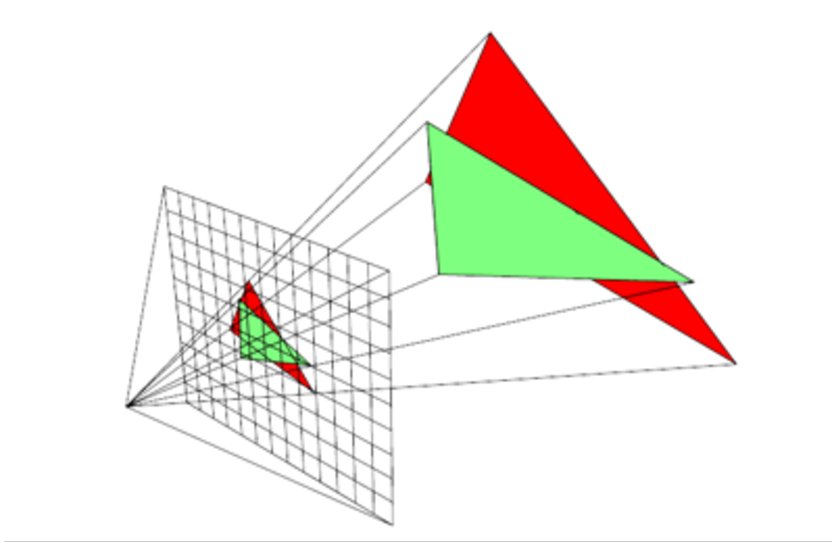
\includegraphics[width=0.47\textwidth]{rasterization.pdf}
  \hspace{\fill}
  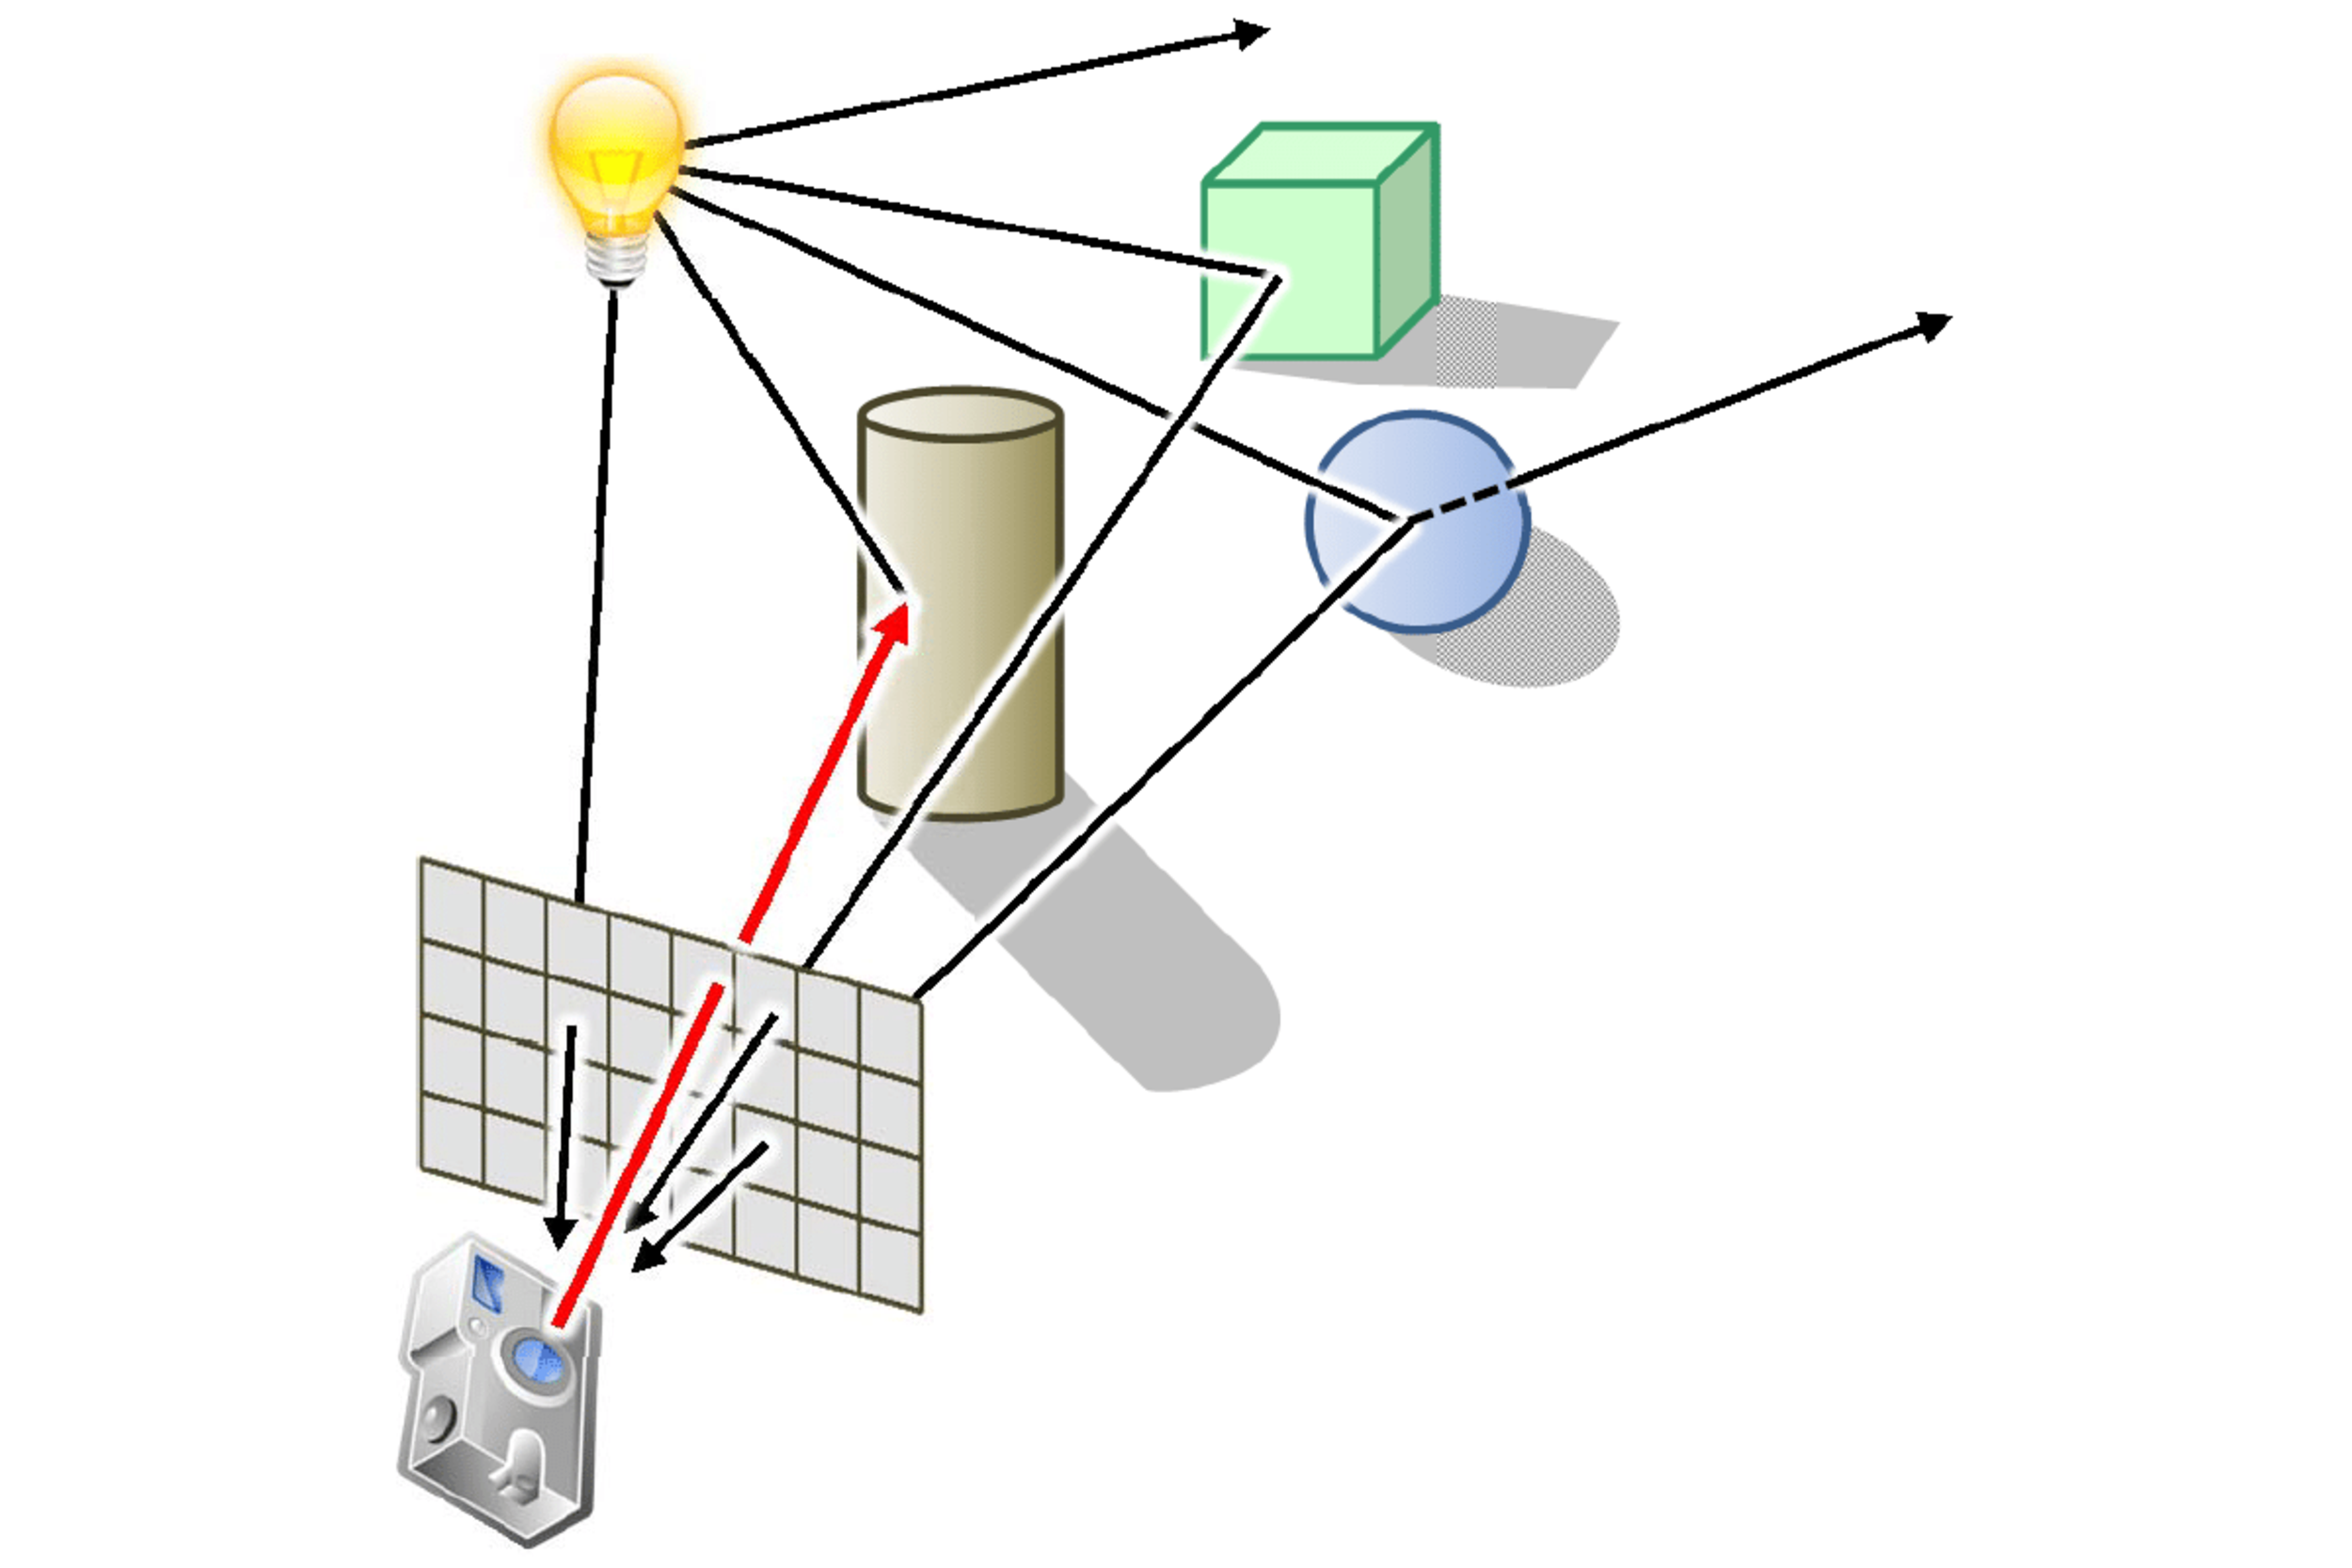
\includegraphics[width=0.47\textwidth]{raytracing.pdf}
  \caption{光栅化和光线追踪示意图}
  \label{fig:rasterization}
\end{figure}

与渲染相对应,逆渲染也是计算机图形学中的一个重要问题。它的主要目标是从提供的图像中推断出物体和场景的三维结构和材质、光照等。逆渲染和传统渲染是恰好相反的两个问题。传统渲染利用场景的三维几何、材质、纹理和光照信息来模拟光线交互,从而生成给定视角下观察得到的二维图像;逆渲染则致力于从一个或多个二维图像中重建物体或场景的三维几何、材质、纹理和光照信息。

三维重建是指从一组或多组图像中恢复出三维场景的几何结构和外观信息的过程。从描述中可以看出,三维重建和逆渲染是非常近似的两个概念。可以认为,三维重建是计算机视觉领域通常习惯的称呼,而逆渲染则是计算机图形学领域的术语。也由于这个区别,三维重建通常更关注物体和场景几何信息的恢复,以及视觉效果上的逼真程度,而逆渲染更注重更为底层的材质和光照信息。

由于三维重建和逆渲染问题的重要性,目前已经存在丰富多样的三维重建算法。主流的重建算法大致可以分为两类:基于视觉几何的传统三维重建和基于深度学习的三维重建。

传统的三维重建主要通过多视角的图像对采集数据的相机位姿进行估计,在通过图像提取特征后,借助深度估计等技术完成从二维图像到三维物体的转换。传统的三维重建算法包括 SfM \cite{SfM}、COLMAP \cite{COLMAP1,COLMAP2} 等。

深度学习出现后,大量将其应用于三维重建的算法也纷纷涌现。有些算法将深度学习和传统三维重建结合,改进传统算法中的某些模块,例如 DeepVO \cite{DeepVO}、BA-Net \cite{BA-Net} 等。更多工作则是直接通过深度学习进行三维重建。NeRF \cite{nerf} 将神经辐射场和体渲染相结合,对三维空间中的色彩和密度进行隐式建模,从而实现高质量的新视角合成。3D Gaussian Splatting \cite{3DGS} 是一种基于体素的三维重建方法,并借助可微光栅化,控制每一个体素对应 3D Gaussian 的形状和大小,实现对三维场景的重建。由于深度学习方法重建质量高、效果好,很快成为了三维重建领域的主要研究方向,神经辐射场和 Gaussian splatting 也很快成为了三维重建中的主要表示形式。

\begin{figure}[htbp]
  \centering
  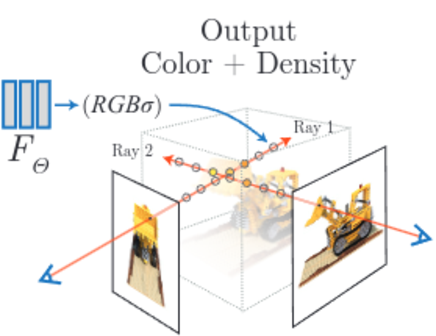
\includegraphics[width=0.47\textwidth]{nerf.pdf}
  \hspace{\fill}
  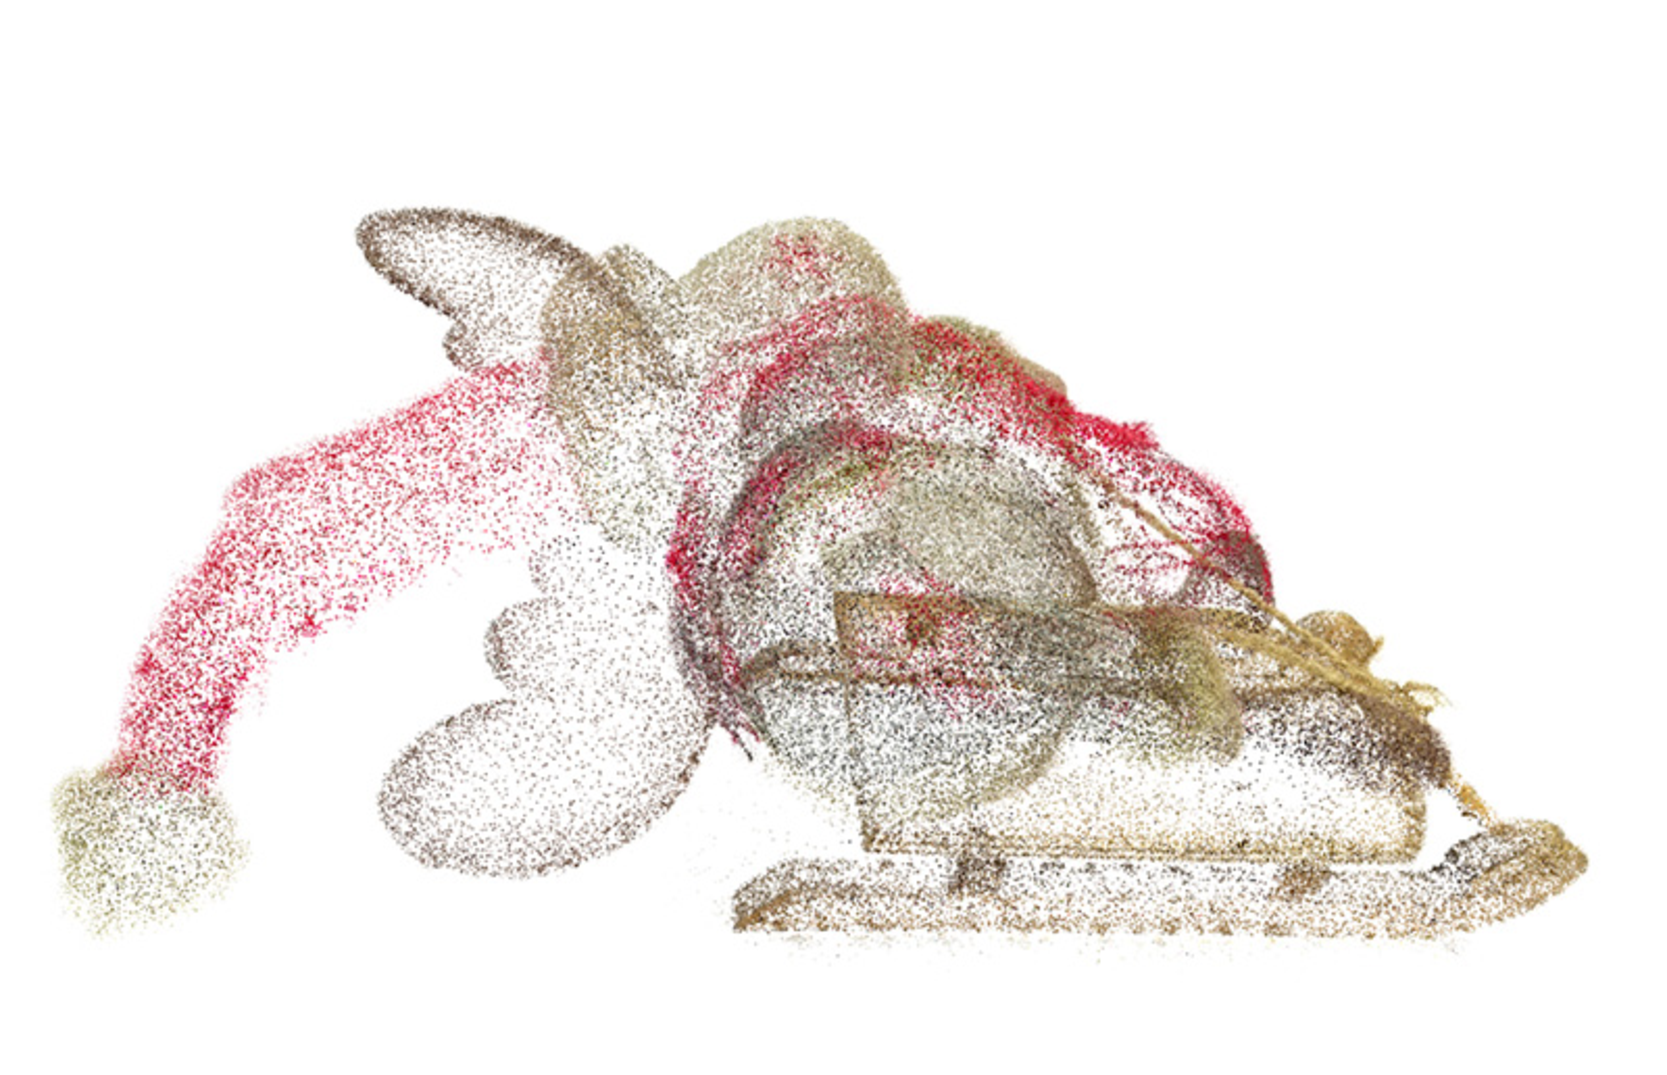
\includegraphics[width=0.47\textwidth]{3dgs.pdf}
  \caption{NeRF 和 3DGS 示意图}
  \label{fig:nerf-3dgs}
\end{figure}

如图 \ref{fig:nerf-3dgs},左图代表 NeRF,右图代表 3D Gaussian splatting。NeRF 采用神经辐射场和体渲染,而3D Gaussian splatting则通过空间中一系列椭球形三维高斯来模拟整个场景。

然而,这些方法也存在问题。无论是神经辐射场或是三维高斯,都属于隐式的几何建模,和传统的显示三维网格(mesh)表示形式有着较大的区别。我们可以通过隐式表示得到漂亮的视觉效果和高质量的新视角合成,但无法得到物体的精确几何信息,不利于下游任务。因此,许多后续工作致力于将这些隐式建模转换为显示的三维网格表示,例如 nvdiffrec \cite{nvdiffrec}、Nerf2Mesh \cite{Nerf2Mesh} 等等。

另一个重要的问题在于如何还原精确的材质和光照信息。NeRF 等一系列相关工作都致力于新视角合成问题,能够在新颖视角下生成极其真实的图像。然而,NeRF 采用的体渲染方法将材质和光照信息烘焙在神经辐射场中,并没有提取显式的材质和光照表示。一些工作尝试通过额外的网络结构来还原材质和光照信息,例如 TensoIR \cite{tensoir} 在 TensoRF \cite{tensorf} 的基础上,通过多层感知机(MLP)从外观特征中提取材质信息,并通过基于物理的可微渲染,在更新密度场的同时更新材质和光照。然而,这些工作大多使用可微光栅化或是简化版的光线追踪,并通过一些额外网络来拟合间接光照。这就导致了他们不能准确地计算全局光照的效果,也不能真实的还原光线和物体或场景的交互。

此外,逆渲染问题本身也是一个不适定(ill-posed)问题。对于给定的单张图像,可能存在多组场景参数与之对应。当输入多张不同角度的图像时,逆渲染问题的解可能会更加稳定,但不适定性仍然存在。一个经典的问题是对于阴影的处理。常见图像的 RGB 空间都是在区间 $[0, 255]$ 中的整数,离散的颜色值意味着在渲染时需要进行取整或截断。而黑色阴影部分对应的 RGB 值太小,可能导致严重的信息丢失。在不使用光线追踪的情况下,我们无法准确地模拟阴影的效果,这就导致许多逆渲染方法会在重建的材质中出现照明伪影。也有一些工作尝试去除这些伪影,例如 SIRe-IR \cite{SIRe-IR} 针对强光环境下的伪影问题,通过同时建模间接辐射场、法线、可见性和直射光,消除材质中的阴影和间接照明,而不会对场景施加严格的约束。但通过可见性来处理伪影的方法仍旧不如光线追踪来得直接有效和准确,并且通过球形高斯来模拟直接和间接光照并不能很好地处理各向异性材质,因此他们无法将金属材质引入考虑范围。

然而,将光线追踪引入三维重建和逆渲染也存在不少困难。想要通过神经网络优化的关键条件是能够计算梯度,而在光线追踪中,我们很难计算渲染结果关于几何的梯度。这是因为光线和物体相交与否是一个不连续的过程,我们难以处理在物体边界处的情形。现有的可微光线追踪方法主要致力于如何计算渲染结果关于几何梯度,并通过神经网络训练优化场景的各个参数。但这些方法大多只能调整三维几何形状的位置大小,而不能生成和删除几何网格,因而往往需要一个合适的几何初始化。但光线追踪可以帮助我们准确地模拟全局光照效果,从而消除重建的材质中的照明伪影,得到更真实的纹理和材质信息。因此,将其引入三维重建和逆渲染中,是一个困难但有意义的任务。

\section{研究内容}

由于可微光线追踪难以处理几何梯度,本文试图通过结合现有的三维重建方法,结合可微光栅化和可微光线追踪,在良好几何结构的基础上,通过光线追踪优化材质和环境照明,以期减少重建的材质中的照明伪影,得到更真实的纹理和材质信息。总的来说,本文的贡献如下:

1. 与现有的逆渲染方法不同,我们的模型重建了一个高质量的水密流形三维网格;

2. 我们的模型同时优化几何、纹理和光照,生成的结果可以方便地应用于下游任务,如重新照明、物理模拟、材质编辑等;

3. 我们的模型同时利用可微分光栅化和可微分光线追踪,恢复了接近现实的材质和光照信息。这种方法有效地减少了材质和纹理中次要光照的照明伪影。

\section{论文组织结构}

本文的结构将按照如下顺序组织:

第二章:相关工作。介绍当前主流的三维重建和逆渲染方法,以及可微光线追踪方法。

第三章:研究方法。详细阐述我们的逆渲染框架和流程,包括 TensoIR 的训练、可微光栅化和可微光线追踪的设计。

第四章:实验结果。首先介绍本文实验采用的数据集和评价标准,以及实验环境和设置,然后展示实验结果和分析,证明第三章介绍的方法的有效性。

第五章:总结和展望。总结本文的工作,指出存在的问题和不足,并展望未来的研究方向。
